\section{DETERMINING THE ONLINE OBSERVABILITY OF BCNs}

In this paper we proposed two ways to determine the online observability of {\em BCNs}, the first one is by supertree; the second one is by directed graph. The construction process of supertree simulates deduction process mentioned before. Then we check the tree based on the definition of online observability of \BCNs\ depth first or breadth first. When we used the super tree to determine the observability of {\em BCNs}, we need to check the existence of loops, and many nodes in the tree are repeated, which will take a lot of time overhead and space overhead. So we proposed the second way which determine the online observability by directed graph,   in this way we can avoid checking the existence of loop and avoid checking repeated nodes. There are also other advantages like determining observability earlier and select the input smarter, which will reduce time and space overhead.    

\subsection{Supertree} As we mentioned before when we want to determine the initial state of {\em BCNs}, we can use the deduce function. Then according to the definition of online observability we will alternately observing the output and deciding the input. When the  cardinal number of the states set comes into be $1$ we can determine the initial state, and stop deducing the initial state of {\em BCNs}. According to this process, we can define the supertree for {\em BCNs}. For convenience, we use the states set inside the node to represent the node, and output in the edge to represent the edge.
\begin{definition}[Supertree]
The root node of the supertree should be $\Delta_N$, if ($|S_i|=1$) then $S_i$ would be the leave node, else if a node $S_i$ in the $2k + 1$ ($k\ge 0$) layer of the supertree, then its son nodes would be $D\left(S_i,\varepsilon, O_i\right)$, $O_i$ would be the edge from $S_i$ to $D\left(S_i,\varepsilon, O_i\right)$ where $|D\left(S_i,\varepsilon, O_i\right)|>0$, if a node $S_i$ in the $2k + 2$ ($k\ge 0$) layer of the supertree, then its son nodes would be $D\left(S_i,I_i,\varepsilon\right)$ where $|D\left(S_i,\varepsilon, O_i\right)|>0$, $I_i$ would be the edge from $S_i$ to $D\left(S_i,I_i,\varepsilon\right)$. 
\end{definition}

  \begin{figure}[thpb]
      \centering
      \framebox{\parbox{3in}{
		\centerline{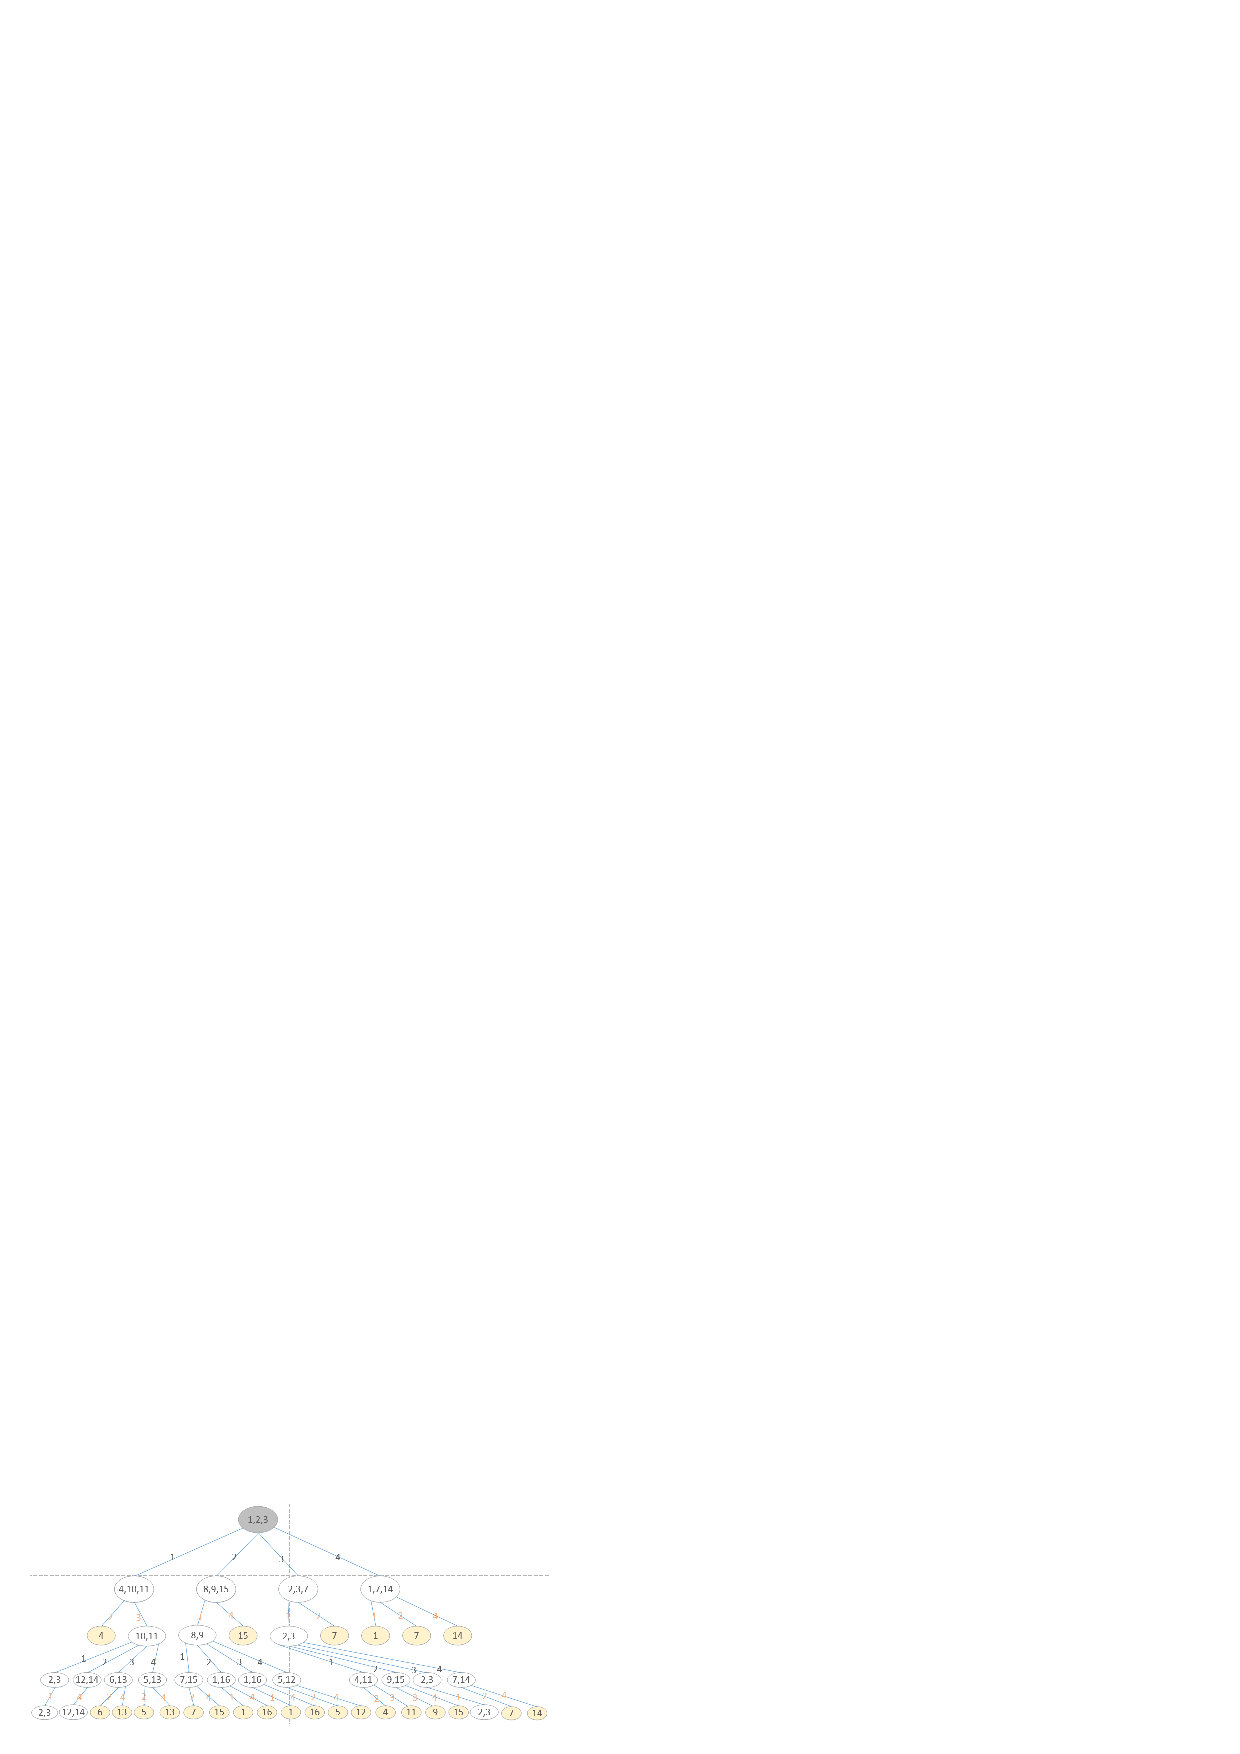
\includegraphics[scale=0.067]{figures/Fig3.png}}
	}}
      
      \caption{Branch of the tree which represents $\{\delta_{16}^1,\delta_{16}^2,\delta_{16}^3\}$. The blue edges and orange edges show the observing output processes and deciding input processes respectively; the yellow nodes are leaf nodes.}
      \label{fig:3}
   \end{figure}

For example, the Fig.\ref{fig:3} show branch of the tree which represents $\{\delta_{16}^1,\delta_{16}^2,\delta_{16}^3\}$, the nodes represent the states sets, the blue edges represent the observing output processes, and the orange edges represent the deciding input processes. And only the yellow nodes are the leave nodes, so you can see that this branch is not completed. If we want to find all of the ways to determine the initial state, we have to build the complete tree, it will takes many additional time and space overhead. Especially when there are loops in the tree like the $\{\delta_{16}^2,\delta_{16}^3\}$ in fourth layer and the $\{\delta_{16}^2,\delta_{16}^3\}$ in fifth layer that will form a loop. In this case you can never build the complete tree, so you need to check the existence of loops and omit it. There are also some nodes take the same states set which will also take additional overhead, like that there two nodes which take $\{\delta_{16}^1,\delta_{16}^{16}\}$ in the fifth layer. But if we only need to find a ways to determine the initial state, when we find the leaf nodes $\delta_{16}^1$, $\delta_{16}^7$ and  $\delta_{16}^{14}$ in third layer by breadth-first algorithm, you can make sure that the states set $\{\delta_{16}^1,\delta_{16}^2,\delta_{16}^3\}$ is 1 step deterministic.  
\subsection{Directed Graph}
To improve the shortcomings of the way by supertree, we proposed the way by derected graph wich takes less time and space overhead. The most difference between supertree and derected graph is that supertree is built from the root node to leaf nodes, but the derected graph is built from smaller nodes (contain less states) to larger nodes (contain more states). 

The construction algorithm of derected graph is shown in the Algorithm.\ref{alg:1}, the algorithm to build nodes used in the Algorithm.\ref{alg:1} is shown in the Algorithm.\ref{alg:2}. Some details in Algorithm.\ref{alg:1} and Algorithm.\ref{alg:2} are as follows:
\begin{itemize}
 \item Sort the states inside the nodes, and then sort the nodes: For example, the nodes $\{\delta_{16}^1,\delta_{16}^2\}$, $\{\delta_{16}^1,\delta_{16}^3\}$ and $\{\delta_{16}^2,\delta_{16}^3\}$ shown in Fig.\ref{fig:4}. 
  \item Using other nodes to find the suitable inputs set for nodes with $k$ states: For example, we can search inputs sets which make $\{\delta_{16}^4,\delta_{16}^5,\delta_{16}^6\}$, $\{\delta_{16}^5,\delta_{16}^6,\delta_{16}^7\}$ and $\{\delta_{16}^4,\delta_{16}^7\}$ $z$ ($z\ge0$) steps deterministic, and then take the intersection of these sets to be the suitable inputs set of $\{\delta_{16}^4,\delta_{16}^5,\delta_{16}^6,\delta_{16}^7\}$. 
  \item Check whether an input can make a nodes $z$ steps deterministic: According to the order determined in previous steps, we check every node one by one. If for one input $I_i$ which belongs to suitable inputs set of the states set $S_i$ implies $|D\left(S_i,I_i,\varepsilon\right)|<|S_i|$, we can make sure the $I_i$ is a wrong input; else if for all $O_i \in \Delta_Q$ and $|D\left(S_i,I_i,O_i\right)|>0$, the $D\left(S_i,I_i,O_i\right)$ is $z$ steps deterministic then $I_i$ is a right input, then connect the node $S_i$ to all nodes $D\left(S_i,I_i,O_i\right)$ with directed edges, the colour of directed edges represent the corresponding input; else if there exist $O_i \in \Delta_Q$ and we can not make sure whether $D\left(S_i,I_i,O_i\right)$ is $z$ steps deterministic, we check it in the next round. 
\end{itemize} 

\begin{algorithm}[h]
\caption{Algorithm to construct the directed graph of BCNs}
\begin{algorithmic}[1]
\REQUIRE 
The algebraic forms of BCN
\ENSURE  
The directed graph of BCN
\STATE Define a int variable $k=0$, to represent the number of states in the nodes.\
\STATE Define a boolean type variable $Ob=0$, to represent the online observability of BCN.\
\WHILE {buildnode(k)==1}
\STATE $k= k+1$
\IF{$k==2$}
\STATE We make $\Delta_M$ as the suitable inputs set for every node with $k$ states.
\ELSE
\IF{$k>2$}
\STATE We use two nodes with $(k-1)$ states and a node with two states to find the suitable inputs set for every node with $k$ states. 
\ENDIF
\ENDIF
\FOR{every node with $k$ states}
\FOR{every input in the suitable input set of the nodes}
\STATE Check whether this input can make the nodes $z$ ($z\ge0$) steps deterministic, and build edges for this node.
\ENDFOR
\ENDFOR
\IF {there exist one node without any edge connect it with other nodes}
\STATE $Ob=0$ return Ob
\ENDIF
\ENDWHILE
\STATE $Ob=1$ return Ob
\end{algorithmic}
 \label{alg:1}
\end{algorithm}

\begin{algorithm}[h]
\caption{Algorithm to build nodes with $k$ states}
\begin{algorithmic}[1]
\REQUIRE 
The number of states in the nodes $p$
\ENSURE  
The nodes with $p$ states
\STATE int buildnode(int p)
\STATE  \{ 
\STATE $p=p+1$\
\STATE  Try to build all the nodes with $p$ states whose corresponding outputs are the same, and classify them by their corresponding outputs.\
\IF{Failed to build} 
\STATE  return 0;
\ELSE 
\STATE Sort the states inside the nodes from small to large, and then sort the nodes based on the values inside the nodes. %(For example, the nodes $\{\delta_{16}^1,\delta_{16}^2\}$, $\{\delta_{16}^1,\delta_{16}^3\}$ and $\{\delta_{16}^2,\delta_{16}^3\}$ shown in {\em Fig.\ref{fig:4}}. )
\STATE return 1;
\ENDIF 
\STATE \}
\end{algorithmic}
 \label{alg:2}
\end{algorithm}

According the construction process, we have the definition of directed graph.
\begin{definition}[Directed Graph]
For every node $S_j$ in the directed graph, there exists $ k \ge 0$ implies $S_j$ is $k$ stepes deterministic; for every distinct two $s_a, s_b \in S_i$ we have $Hs_a=Hs_b$; if $|S_i|=1$ there are not edge from it to other nodes, else if there are exist one edge $I'$ from it to one nodes then there exist $p$ ($p\ge 1)$ edges contain $I'$ from it to nodes $S_1,\cdots,S_p$ that \[|S_j|= |S_1|+,\cdots,|S_p|\] and \[D\left(S_j,I',\varepsilon\right)=S_1\vee,\cdots,\vee S_p.\]
\end{definition}

We can also use the directed graph to determine the existed second and fourth kinds of observability. When we trying to build bottom layer and penultimate layer of the directed graph, and if there are exist some nodes in penultimate layer has no edges from it to other nodes, then this BCN is not satisfied existed second observability. When we trying to build edges for every layer, and is there exist one node whose right inputs set is not $\Delta_M$, then this BCN is not satisfied existed fourth observability.
\begin{figure}[thpb]
      \centering
      \framebox{\parbox{3in}{
		\centerline{\includegraphics[scale=0.090]{figures/Fig4.png}}
	}}
      
      \caption{Part of the directed graph which represents $\{\delta_{16}^1,\delta_{16}^2\}$, $\{\delta_{16}^1,\delta_{16}^3\}$ and $\{\delta_{16}^2,\delta_{16}^3\}$. The green, black, orange, blue edges show the inputs $\delta_4^1$, $\delta_4^2$, $\delta_4^3$ and $\delta_4^4$ respectively.}
      \label{fig:4}
   \end{figure}
\subsection{Complexity Analysis}
The way use the directed graph to determine the online observability of \BCNs\ is better than by supertree, so we analyze the complexity of it. We classify the states with their corresponding output and form the set of states with the same corresponding output: $S_1$, $S_2$,...,$S_M$.

Firstly, we need to calculate the upper bound of the number of the states in a directed graph nodes $k$, then :
\begin{equation}
\begin{split}
k_{upb}= Max(|S_1|,|S_2|,\cdots,|S_M|)
\end{split}
\end{equation}

Secondly, the number of each nodes with $k$ states:
\begin{equation}
\begin{split}
k_{non}= C_{|S_i|}^k+\cdots +C_{|S_p|}^k
\end{split}
\end{equation}
where $|S_i|,\cdots,|S_p|\ge k$.

And then the the cardinal number of suitable inputs set of each node, and the time used to check each input is a right input for a node. Finally, calculate the complexity by layer by layer. But the cardinal number of suitable inputs set of a node depends on the number of the states in it, and the other three nodes which used to find the suitable inputs set for it. And the time used to check an input is a right input for  a node of directed graph also depends on the update rules of the {\em BCNs}. So it is hard to give a accurate complexity of the algorithm without the complete imformation of {\em BCNs}.

We can use other three nodes like $\{\delta_{16}^4,\delta_{16}^5,\delta_{16}^6\}$, $\{\delta_{16}^5,\delta_{16}^6,\delta_{16}^7\}$ and $\{\delta_{16}^4,\delta_{16}^7\}$ which is $z$ ($z\ge0$) steps deterministic to find suitable inputs set for $\{\delta_{16}^4,\delta_{16}^5,\delta_{16}^6,\delta_{16}^7\}$. Because only the input which make the subset of $\{\delta_{16}^4,\delta_{16}^5,\delta_{16}^6,\delta_{16}^7\}$ $z$ steps deterministic will make the $\{\delta_{16}^4,\delta_{16}^5,\delta_{16}^6,\delta_{16}^7\}$ $z$ steps deterministic, and use the this three nodes will be a convenient way to cover all the subset of $\{\delta_{16}^4,\delta_{16}^5,\delta_{16}^6,\delta_{16}^7\}$ which with cardinal number 2. By this way we can  reduce the cardinal number of suitable inputs set for every nodes with more than 2 states, then reduce the time cost. 
%Because the states in a nodes will have the same corresponding output, so we have the upper bound of the number of the states in a directed graph nodes $k$: We classify the states with their corresponding output and form the set of states with the same corresponding output, the greatest cardinal number of these set would be the upper bound of $k$. 